% First full draft (November 2026).  Venue-neutral article layout; swap the preamble for the venue template.
% Build: cd paper && latexmk -pdf main.tex     Figures: python3 scripts/paper_figures.py (from the repository root)
\documentclass[11pt,a4paper]{article}
\usepackage[utf8]{inputenc}
\usepackage[T1]{fontenc}
\usepackage[margin=2.5cm]{geometry}
\usepackage{amsmath,amssymb,amsthm}
\usepackage{graphicx}
\usepackage{booktabs}
\usepackage{mathptmx}
\usepackage[round,authoryear]{natbib}
\usepackage[colorlinks=true,linkcolor=blue!50!black,citecolor=blue!50!black,urlcolor=blue!50!black]{hyperref}
\usepackage{xcolor}
\usepackage{caption}
\captionsetup{font=small,labelfont=bf}

\newtheorem{proposition}{Proposition}
\newcommand{\tri}{\operatorname{tri}}
\newcommand{\clip}{\operatorname{clip}}
\newcommand{\todo}[1]{\textcolor{red}{[#1]}}

\title{Beyond Bounded Weights: Non-Saturating Periodic Reparameterization\\for Preserving Plasticity in Continual Learning}
\author{Ahmet \c{S}ahin \c{C}ak{\i}r \and E.~U.~K\"u\c{c}\"uksille\\[2pt]
\small \todo{affiliation and e-mail addresses}}
\date{}

\begin{document}
\maketitle

\begin{abstract}
Neural networks trained on a long sequence of tasks gradually lose the ability to learn new ones.
Growth of the weight magnitude is one of the identified causes, and keeping every weight inside a fixed
interval is a simple and effective remedy.
We ask whether boundedness alone is what matters.
We study structural reparameterizations $W = A\,f(\Theta/A)$ in which a bounded map $f$ guarantees $|W|\le A$
by construction, and compare a smooth periodic map (sine), a smooth non-periodic map (tanh) and a
piecewise-linear periodic map (triangle wave).
On Online Permuted MNIST at the canonical length of 800 tasks with 60{,}000 examples each, with ten paired seeds,
the smooth maps do not preserve plasticity: the sine map ends \emph{below} the unconstrained network
(normalized area under the online-accuracy curve $0.818$ versus $0.856$) and tanh matches it ($0.859$).
Their weights drift towards the bound, where the derivative of the map vanishes; the effective step size falls
to about $11\%$ of its initial value and $79\%$ of the parameters end up saturated.
The triangle wave, whose derivative has unit magnitude everywhere, shows no measurable loss over 800 tasks
($0.939$), outperforms layer normalization with weight decay ($0.925$), and is statistically equivalent to
weight clipping under a pre-specified margin of $0.005$ on all four metrics we test.
A causal intervention supports the explanation: keeping the sine map in the forward pass but replacing its
derivative by its sign in the backward pass restores performance from $0.818$ to $0.924$.
Element-wise boundedness is therefore not sufficient; the map must also keep the update magnitude away from zero.
We also report where the conclusion stops holding: under Adam the ranking of hard and smooth bounds reverses,
and in a wide network that does not lose plasticity none of the bounded maps helps.
\end{abstract}

% ======================================================================================================
\section{Introduction}

A network that is trained continually, on a stream of tasks that never ends, should learn the thousandth task
as well as the first. Standard deep learning does not: after enough tasks a network trained with
backpropagation learns new tasks more slowly and less accurately than a freshly initialized copy
\citep{ash2020warm,dohare2021continual,lyle2023understanding,dohare2024loss}. This \emph{loss of plasticity}
is distinct from catastrophic forgetting, which concerns old tasks; it concerns the ability to acquire new ones.

Several mechanisms have been tied to the phenomenon, among them dead or dormant units
\citep{sokar2023dormant,abbas2023loss}, loss of representational rank \citep{lyle2022understanding},
changes in curvature \citep{lewandowski2023directions} and growth of the parameter norm
\citep{lyle2023understanding,dohare2024loss}; they act together, and treating a single one is usually not
enough \citep{lyle2024disentangling}. Among the remedies that target the parameter norm, the simplest is
\emph{weight clipping} \citep{elsayed2024weight}: after every update each weight is projected back onto an
interval $[-\kappa b,\kappa b]$ whose width is tied to the initialization scale $b$ of its layer.

Clipping is an operation applied \emph{after} the optimizer step. The same constraint can be imposed
\emph{structurally}, by writing each weight as a bounded function of an unconstrained parameter,
\begin{equation}
  W \;=\; A\, f\!\left(\Theta/A\right), \qquad f:\mathbb{R}\to[-1,1], \label{eq:reparam}
\end{equation}
so that $|W|\le A$ holds for every value of $\Theta$ and no projection is needed. This is attractive: the
constraint is part of the model, it composes with any optimizer, and a periodic $f$ gives a parameter that
has left the interval a way back in. Our starting hypothesis was that the smooth periodic choice
$f=\sin$ would preserve plasticity because it keeps the weights bounded.

The hypothesis fails, and the way in which it fails is the subject of this paper. Under gradient descent on
$\Theta$ the change of the effective weight is scaled by $f'(\Theta/A)^2$. A smooth map that attains its bound
has $f'=0$ there, so a weight that approaches the bound receives ever smaller updates and eventually
stops moving. Over a long stream this happens to most of the network. The remedy follows from the diagnosis:
use a bounded periodic map whose derivative never vanishes. The triangle wave is the simplest such map; inside
the interval it is the identity, and at the bound the parameter is \emph{reflected} instead of frozen.

\paragraph{Contributions.}
\begin{itemize}
  \item We show, at the canonical stream length of \citet{dohare2024loss} and with ten paired seeds, that
        bounded weights obtained through a smooth map do not preserve plasticity: the sine map is worse than
        the unconstrained network in every one of the ten seeds, and tanh is equivalent to it in normalized
        area under the curve (Section~\ref{sec:main}).
  \item We identify the cause as Jacobian damping at the bound, measure it (saturated fraction, step multiplier,
        distance to the bound; Section~\ref{sec:mechanism}), and test it with an intervention that removes the
        damping while leaving the forward map unchanged (Section~\ref{sec:causal}).
  \item We show that a non-saturating periodic map, the triangle wave, preserves plasticity over 800 tasks
        and is statistically equivalent to weight clipping under a pre-specified margin (two one-sided tests),
        and that both outperform layer normalization with weight decay (Sections~\ref{sec:main}--\ref{sec:lnwd}).
  \item We delimit the result: sensitivity to the width of the bound, a second benchmark, the Adam optimizer and
        a wide network are reported in Section~\ref{sec:scope}, including the cases in which the ranking changes.
\end{itemize}

We do not claim that the triangle wave improves on weight clipping; in the regime we study the two are
indistinguishable, and we explain why they should be. The claim is about \emph{which property} of a bounded
parameterization matters: not boundedness alone, but boundedness together with an update magnitude that
stays away from zero.

% ======================================================================================================
\section{Related work}

\paragraph{Loss of plasticity.}
Warm-started networks generalize worse than freshly initialized ones \citep{ash2020warm,berariu2021study},
and the effect accumulates over long task sequences until a deep network learns no better than a linear one
\citep{dohare2021continual,dohare2024loss}. The same degradation appears in reinforcement learning, where the
data distribution changes with the policy
\citep{nikishin2022primacy,lyle2022understanding,abbas2023loss,sokar2023dormant,juliani2024study};
\citet{klein2024survey} survey this literature. Explanations include saturated and dead units
\citep{sokar2023dormant,abbas2023loss}, mutually frozen weights \citep{zilly2021plasticity}, loss of
curvature directions \citep{lewandowski2023directions}, feature-rank collapse \citep{lyle2022understanding}
and norm growth \citep{lyle2023understanding}. Recent analyses describe loss of plasticity as trapping in
invariant manifolds of the gradient flow \citep{joudaki2026barriers}, separate it into regimes with different
signatures \citep{wang2025dual}, or attribute part of it to the abruptness of task changes
\citep{liu2026gradually}. \citet{lyle2024disentangling} show that the mechanisms are largely independent and
that combining layer normalization with weight decay addresses several of them at once.

\paragraph{Controlling weight magnitude.}
Methods that act on the parameter norm include $L^2$ regularization towards zero or towards the initial
parameters \citep{kumar2023maintaining}, shrink-and-perturb \citep{ash2020warm}, projection of the weight norm
after normalization \citep{lyle2024normalization}, hyperspherical normalization \citep{lee2025hyperspherical},
soft rescaling \citep{oh2025soft}, spectral and orthogonality regularizers
\citep{lewandowski2025spectral,chung2024parseval} and weight clipping \citep{elsayed2024weight}.
Clipping weights to a fixed interval has a longer history outside continual learning, for example in
networks with binary weights \citep{courbariaux2015binaryconnect}. Other families of methods reinitialize
units or parameters \citep{dohare2024loss,sokar2023dormant,nikishin2022primacy,farias2025self,galashov2024nonstationary}
or perturb them according to their utility \citep{elsayed2024addressing}. Our work stays within the first
family and asks what a magnitude constraint must look like in order to help.

\paragraph{Periodic functions and plasticity.}
Periodic \emph{activations} are established in implicit neural representations \citep{sitzmann2020implicit}
and for extrapolating periodic signals \citep{ziyin2020neural}. In continual learning,
\citet{lewandowski2025fourier} show that concatenated sine and cosine activations in every layer keep networks
trainable, and \citet{lillo2026activation} relate plasticity to the shape of the activation function,
in particular to a non-zero derivative floor. \citet{chen2025intrinsic} report that quantum neural networks,
whose parameters live on a compact manifold, do not lose plasticity, while a classical network with sine
activations does. All of these change the function computed by a unit. We instead apply the periodic map to
the \emph{weights}: the network remains a standard ReLU network with respect to $W$, and only the coordinates
in which the optimizer moves are changed. Periodic functions of the weights have been used as regularizers for
quantization \citep{naumov2018periodic}, and a triangle-wave map has been used to impose periodicity in a
neural shape parameterization \citep{dai2025shaping}; we are not aware of a study of bounded periodic weight
reparameterizations for loss of plasticity.
% TODO before submission: re-read Dai et al. (2025) and quote the triangle-wave passage and its remark on sine gradients exactly.

\paragraph{Reparameterization and straight-through gradients.}
Writing weights as a function of other parameters changes the optimization geometry without changing the
function class \citep{salimans2016weight}. The intervention of Section~\ref{sec:causal} replaces the derivative
of the map in the backward pass and is a straight-through estimator in the sense of \citet{bengio2013estimating}.

% ======================================================================================================
\section{Bounded reparameterizations}\label{sec:method}

\subsection{Definition}

Consider a fully connected layer with fan-in $n$ and weights initialized uniformly in $[-b,b]$ with the
Kaiming bound $b=\sqrt{6/n}$ \citep{he2015delving}. We fix an amplitude $A=\gamma b$ with $\gamma\ge 1$ and
parameterize every weight (and every bias, with $A_{\mathrm{bias}}=\gamma/\sqrt{n}$) by a free parameter
$\Theta$ through Eq.~\eqref{eq:reparam}. We consider three maps (Figure~\ref{fig:maps}):
\begin{align}
  \text{sine:}\quad & f(x)=\sin x, & f'(x)&=\cos x,\\
  \text{tanh:}\quad & f(x)=\tanh x, & f'(x)&=1-\tanh^2 x,\\
  \text{triangle wave:}\quad & f(x)=\tri(x)=\tfrac{2}{\pi}\arcsin\!\big(\sin(\tfrac{\pi}{2}x)\big), & |f'(x)|&=1 .
\end{align}
The triangle wave has period $4$, equals the identity on $[-1,1]$ and is reflected at $\pm1$. Its derivative
is $+1$ on rising and $-1$ on falling flanks; at the corners, a set of measure zero, we use the one-sided
value, so the derivative is never zero.

\paragraph{Matched initialization.} All models start from the same effective weights: we draw $W_0$ once
and set $\Theta_0 = A f^{-1}(W_0/A)$ on the principal branch. Because the argument of $f$ is $\Theta/A$, we
have $\partial W/\partial\Theta=f'(\Theta/A)$, which equals one at $\Theta=0$; a step on $\Theta$ with learning
rate $\eta$ therefore moves a small weight exactly as a step on $W$ would in the standard network.

\begin{figure}[t]
  \centering
  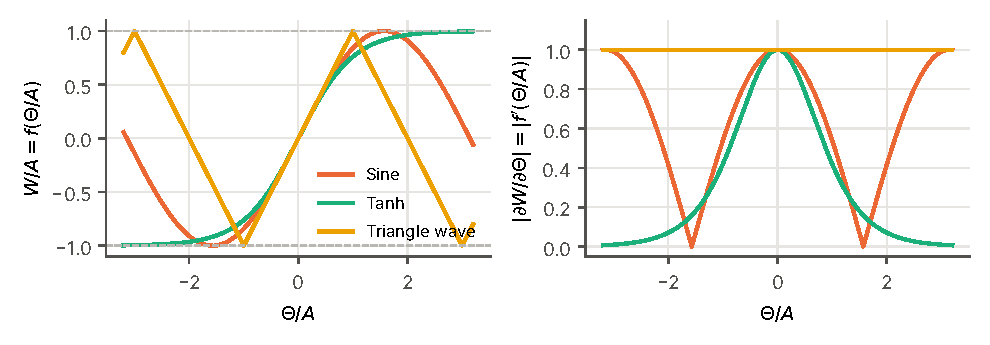
\includegraphics[width=0.88\linewidth]{figures/fig_maps.pdf}
  \caption{The three bounded maps (left) and the magnitude of their derivative (right). The derivative of the
  smooth maps vanishes at the bound; that of the triangle wave has unit magnitude everywhere.}
  \label{fig:maps}
\end{figure}

\subsection{Jacobian damping}

Let $g=\partial L/\partial W$. One step of stochastic gradient descent on $\Theta$ changes the weight, to first
order, by
\begin{equation}
  \Delta W \;\approx\; f'(\Theta/A)\,\Delta\Theta \;=\; -\,\eta\, f'(\Theta/A)^2\, g . \label{eq:damping}
\end{equation}
The factor $f'^2\in[0,1]$ is a per-parameter multiplier of the learning rate. For the sine map
it is $\cos^2(\Theta/A)=1-(W/A)^2$: the closer a weight is to the bound, the smaller its step.

\begin{proposition}\label{prop:tradeoff}
Let $f:\mathbb{R}\to[-1,1]$ be continuously differentiable and attain the value $1$ or $-1$ at some point $x^\star$.
Then $f'(x^\star)=0$. In particular, a map cannot be smooth, bounded with attained bounds, and have a
derivative bounded away from zero.
\end{proposition}
\begin{proof}
$x^\star$ is an interior extremum of a differentiable function.
\end{proof}

The proposition is elementary, but it organizes the design space. A smooth bounded map either attains its
bound (sine), in which case the step multiplier vanishes at a finite $\Theta$ and a parameter that reaches it
stops; or it approaches the bound only asymptotically (tanh), in which case the multiplier decays without
limit as $|\Theta|$ grows. In both cases a weight that the data push towards the bound is slowed down
precisely when it gets there, and noise can move it back only at the reduced rate. We refer to this
one-way accumulation as a \emph{saturation ratchet}. Giving up smoothness removes the trade-off: the triangle
wave is bounded and has $|f'|=1$.

\subsection{Reflection and projection}

For the triangle wave Eq.~\eqref{eq:damping} is exact inside the interval, $\Delta W=-\eta g$. A step
that would carry the weight to $A+\delta$ with $0<\delta<2A$ leaves it at $A-\delta$: the weight is reflected at
the bound. Weight clipping \citep{elsayed2024weight} maps the same step to $A$: the weight is projected.
After one step from a common starting point the two results differ by the overshoot $\delta\le\eta|g|$, and
neither rescales the gradient. When steps are small relative to the width of the interval, a triangle-wave
network and a clipped network with $\kappa=\gamma$ are therefore expected to follow nearly the same
trajectory in $W$; the difference is that the constraint is part of the parameterization instead of a
separate projection step. The two can separate when the step is large relative to the interval, which is the
case for adaptive optimizers (Section~\ref{sec:scope}).

\subsection{Reflected sine: removing the damping without changing the map}\label{sec:floor}

To test whether damping is the cause of failure and not some other property of the sine map, we use an
intervention that leaves the forward pass untouched. In the backward pass we replace $f'$ by
\begin{equation}
  \tilde f'(x) \;=\; \operatorname{sign}\!\big(f'(x)\big)\,\max\!\big(|f'(x)|,\varepsilon\big), \label{eq:floor}
\end{equation}
a straight-through-type estimator \citep{bengio2013estimating}. With $\varepsilon=0$ this is the sine map;
with $\varepsilon=1$ the backward derivative is $\operatorname{sign}(\cos(\Theta/A))$, so a parameter passes
over the crest and comes back down on the other side. We call this variant the \emph{reflected sine}. Its
weights are still $A\sin(\Theta/A)$; only the damping is removed.

% ======================================================================================================
\section{Experimental setup}\label{sec:setup}

\paragraph{Stream.} Online Permuted MNIST \citep{goodfellow2013empirical,zenke2017continual,dohare2024loss}:
every task applies a new random permutation to the pixels of MNIST \citep{lecun1998gradient}. The network sees
each of the 60{,}000 training images of a task once, one image at a time (batch size one), without task
boundaries or task identity, and is evaluated by its \emph{online accuracy}, the fraction of images classified
correctly before the update on them. We use 800 tasks, the length of \citet{dohare2024loss}, which amounts to
$4.8\times10^7$ updates per run.

\paragraph{Network and optimizer.} A ReLU multilayer perceptron with three hidden layers of 100 units, trained
with plain stochastic gradient descent. Wider networks and Adam \citep{kingma2015adam} are treated in
Section~\ref{sec:scope}.

\paragraph{Models.} (i)~The standard network. (ii--iv)~Sine, tanh and triangle-wave reparameterization of all
weights and biases. (v)~Weight clipping with $\kappa=1$ \citep{elsayed2024weight}. (vi)~Layer normalization
\citep{ba2016layer} with weight decay \citep{lyle2024disentangling}. (vii)~The reflected sine
of Section~\ref{sec:floor}.

\paragraph{Hyperparameters.} All hyperparameters were selected on separate development streams of 100 to 200
tasks with 5{,}000 examples per task and were \emph{not} re-tuned for the 800-task stream, for any method
(Appendix~\ref{app:hparams}). The selected values are a learning rate of $0.003$ for all models except the
reflected sine ($0.01$); $\gamma=1.5$ for sine and tanh; $\gamma=1$ for the triangle wave and the reflected
sine; $\kappa=1$ for clipping; and a weight-decay coefficient of $10^{-3}$.

\paragraph{Metrics.} The \emph{normalized AUC} is the mean online accuracy over all tasks. The \emph{early} and
\emph{final windows} are the mean over the first and last 40 tasks, and the \emph{retention ratio} is their
quotient. The \emph{slope} is the linear trend of online accuracy per 100 tasks. The \emph{fresh-model gap} is
the online accuracy of a freshly initialized network trained on the last task minus that of the continually
trained network on the same task; it is positive when the continual learner is worse than a network that has
never seen any other task. We call plasticity \emph{retained} in a run when three conditions hold together:
retention ratio $\ge0.99$, slope $\ge-0.002$ per 100 tasks, and fresh-model gap $\le0.01$. These thresholds
were fixed before the 800-task runs were analysed. As mechanism measures we record the fraction of
\emph{saturated} parameters ($|f'|<0.1$), the mean step multiplier $\langle f'^2\rangle$, the mean distance to
the bound $\langle|W|\rangle/A$, the fraction of dead ReLU units, and the effective rank \citep{roy2007effective}
of the last hidden representation.

\paragraph{Seeds and statistics.} We run ten seeds for models (i)--(vi) and three for the reflected sine, 63 runs
in total. A seed fixes the initialization and the sequence of permutations, so models are compared on
identical streams and all differences are paired. We report means with 95\% $t$-intervals over seeds, paired
differences with 95\% bootstrap intervals \citep{efron1993introduction}, paired $t$-tests, and sign-flip
permutation tests with Holm correction \citep{holm1979simple}. With ten pairs the smallest attainable
permutation $p$-value is $2/2^{10}\approx0.002$. For the comparison between the triangle wave and weight
clipping, absence of a significant difference is not evidence of equality, so we use the two one-sided tests
procedure \citep{schuirmann1987comparison,lakens2017equivalence} with an equivalence margin of
$\Delta=0.005$ in accuracy units, chosen before the ten-seed runs; equivalence is declared when the 90\%
confidence interval of the paired difference lies inside $(-\Delta,\Delta)$.

% ======================================================================================================
\section{Results}

\subsection{Smooth bounds lose plasticity; the triangle wave does not}\label{sec:main}

\begin{figure}[t]
  \centering
  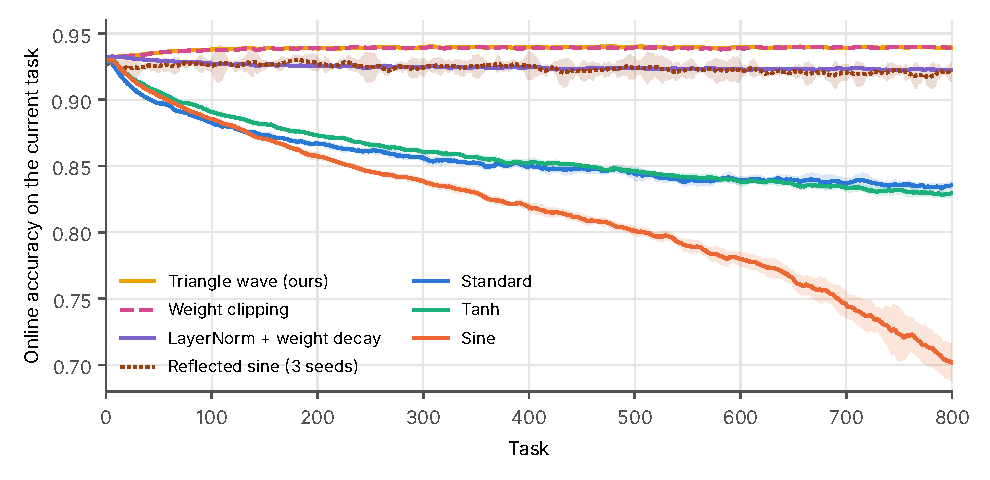
\includegraphics[width=0.92\linewidth]{figures/fig_curves.pdf}
  \caption{Online accuracy on Online Permuted MNIST over 800 tasks of 60{,}000 examples
  (mean over ten seeds, three for the reflected sine; 10-task moving average; bands are 95\% intervals).
  The triangle wave and weight clipping coincide.}
  \label{fig:curves}
\end{figure}

\begin{table}[t]
  \centering\small
  \caption{Online Permuted MNIST, 800 tasks $\times$ 60{,}000 examples, $3\times100$ network, SGD.
  Mean $\pm$ 95\% interval over seeds. Retained: number of seeds that satisfy the three-part criterion of
  Section~\ref{sec:setup}.}
  \label{tab:main}
  \resizebox{\linewidth}{!}{%
  \begin{tabular}{@{}lrccccc@{}}
    \toprule
    Model & $n$ & AUC & Final window & Retention & Fresh-model gap & Retained\\
    \midrule
    Triangle wave (ours)   & 10 & $0.939\pm0.000$ & $0.940\pm0.001$ & $1.005\pm0.001$ & $-0.023\pm0.001$ & 10/10\\
    Weight clipping        & 10 & $0.939\pm0.000$ & $0.940\pm0.001$ & $1.006\pm0.001$ & $-0.022\pm0.003$ & 10/10\\
    LayerNorm + weight decay & 10 & $0.925\pm0.000$ & $0.923\pm0.001$ & $0.992\pm0.001$ & $+0.008\pm0.003$ & 8/10\\
    Reflected sine         &  3 & $0.924\pm0.000$ & $0.920\pm0.001$ & $0.994\pm0.001$ & $+0.005\pm0.014$ & 3/3\\
    Tanh                   & 10 & $0.859\pm0.001$ & $0.831\pm0.002$ & $0.912\pm0.003$ & $+0.085\pm0.003$ & 0/10\\
    Standard               & 10 & $0.856\pm0.001$ & $0.835\pm0.001$ & $0.924\pm0.001$ & $+0.084\pm0.006$ & 0/10\\
    Sine                   & 10 & $0.818\pm0.002$ & $0.720\pm0.012$ & $0.792\pm0.013$ & $+0.212\pm0.015$ & 0/10\\
    \bottomrule
  \end{tabular}}
\end{table}

Figure~\ref{fig:curves} and Table~\ref{tab:main} give the main result. The standard network loses plasticity
steadily: its accuracy falls from $0.901$ in the first hundred tasks to $0.836$ in the last hundred, and at
the end a fresh network is better by $0.084$.

\emph{The sine map makes this worse.} It starts slightly above the standard network (early window $+0.005$)
and then declines at an increasing rate, to $0.724$ in the last hundred tasks. Its AUC is lower than that of
the standard network by $0.039$ (95\% interval $[0.037,0.040]$), with the same sign in all ten seeds
(per-seed differences between $-0.034$ and $-0.043$). \emph{Tanh is no better than no constraint}: its AUC is
within $0.003$ of the standard network, its final window is lower by $0.005$ and its retention ratio by
$0.012$. Bounding the weights with a smooth map therefore does not preserve plasticity; with the sine map it
is harmful.

\emph{The triangle wave shows no loss.} Its accuracy is flat from the second hundred tasks on ($0.939$ to
$0.940$), the slope is $+0.0004$ per 100 tasks, and after 800 tasks it is better than a fresh network by
$0.023$. It satisfies the retention criterion in all ten seeds. Compared with the standard network the AUC
is higher by $0.083$ $[0.082,0.083]$ and the final window by $0.104$ $[0.103,0.105]$; compared with the sine
map, with which it shares boundedness and periodicity, the AUC is higher by $0.121$ $[0.119,0.123]$.
Table~\ref{tab:paired} lists the paired differences.

\begin{table}[t]
  \centering\small
  \caption{Paired differences on identical streams (ten pairs; mean and 95\% bootstrap interval).
  All differences are significant at $p<0.001$ (paired $t$-test) except where a $p$-value is given;
  for tanh $-$ standard, $p=0.002$ (AUC) and $p=0.004$ (final window).}
  \label{tab:paired}
  \resizebox{\linewidth}{!}{%
  \begin{tabular}{@{}lccc@{}}
    \toprule
    Comparison & AUC & Final window & Retention\\
    \midrule
    Triangle $-$ standard & $+0.083\;[+0.082,+0.083]$ & $+0.104\;[+0.103,+0.105]$ & $+0.082\;[+0.081,+0.083]$\\
    Clipping $-$ standard & $+0.082\;[+0.081,+0.083]$ & $+0.104\;[+0.103,+0.105]$ & $+0.082\;[+0.081,+0.083]$\\
    Sine $-$ standard     & $-0.039\;[-0.040,-0.037]$ & $-0.115\;[-0.126,-0.106]$ & $-0.131\;[-0.143,-0.121]$\\
    Tanh $-$ standard     & $+0.003\;[+0.002,+0.004]$ & $-0.005\;[-0.007,-0.003]$ & $-0.012\;[-0.015,-0.010]$\\
    Triangle $-$ sine     & $+0.121\;[+0.119,+0.123]$ & $+0.219\;[+0.210,+0.230]$ & $+0.213\;[+0.203,+0.225]$\\
    Triangle $-$ LN+WD    & $+0.014\;[+0.014,+0.015]$ & $+0.017\;[+0.016,+0.018]$ & $+0.014\;[+0.013,+0.015]$\\
    Triangle $-$ clipping & $+0.0003\;[-0.0000,+0.0006]$ & $-0.0001\;[-0.0006,+0.0005]$ & $-0.0003\;[-0.0015,+0.0009]$\\
                          & $(p=0.09)$ & $(p=0.83)$ & $(p=0.63)$\\
    \bottomrule
  \end{tabular}}
\end{table}

\subsection{The triangle wave is equivalent to weight clipping}\label{sec:tost}

The triangle wave and weight clipping differ by less than $0.0015$ on every metric
(Table~\ref{tab:paired}). To turn ``no detectable difference'' into a positive statement we test equivalence
with the pre-specified margin $\Delta=0.005$ (Table~\ref{tab:tost}). The 90\% interval of the paired difference
lies inside $(-0.003,0.003)$ for all four metrics, so equivalence holds with room to spare and would also hold
for a margin of $0.003$. The two methods agree in the mechanism measures as well: final dead-unit fraction
$0.177$ in both (difference $+0.001$, $p=0.95$), effective rank $54.8$ in both, mean absolute weight $0.071$
in both. This is the behaviour predicted in Section~\ref{sec:method}: with small steps, reflection and
projection at the same bound are nearly the same operation.

\begin{table}[t]
  \centering\small
  \caption{Equivalence of the triangle wave and weight clipping (two one-sided tests, ten paired seeds,
  pre-specified margin $\Delta=0.005$).}
  \label{tab:tost}
  \begin{tabular}{@{}lcccc@{}}
    \toprule
    Metric & Difference & 90\% interval & $p_{\mathrm{TOST}}$ & Decision\\
    \midrule
    Normalized AUC   & $+0.0003$ & $[+0.0000,+0.0006]$ & $<0.001$ & equivalent\\
    Final window     & $-0.0001$ & $[-0.0006,+0.0005]$ & $<0.001$ & equivalent\\
    Retention ratio  & $-0.0003$ & $[-0.0015,+0.0008]$ & $<0.001$ & equivalent\\
    Fresh-model gap  & $-0.0012$ & $[-0.0028,+0.0005]$ & $0.001$  & equivalent\\
    \bottomrule
  \end{tabular}
\end{table}

\subsection{Mechanism: saturation, not dead units}\label{sec:mechanism}

\begin{figure}[t]
  \centering
  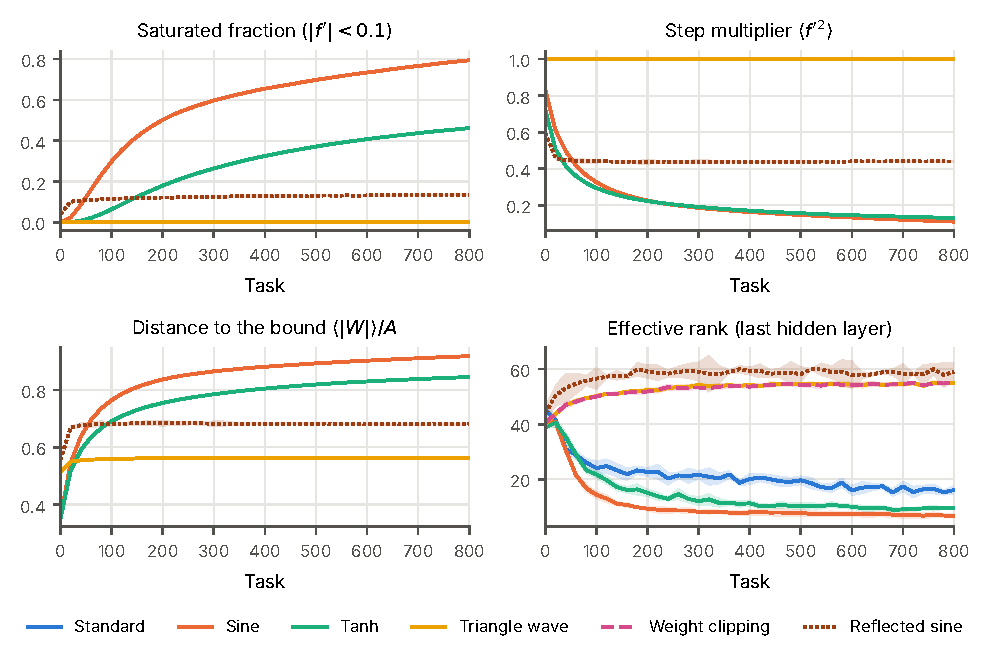
\includegraphics[width=0.9\linewidth]{figures/fig_mechanism.pdf}
  \caption{Mechanism measures over the 800-task stream (mean over seeds, 95\% bands). With the smooth maps the
  weights move towards the bound, the fraction of saturated parameters grows monotonically and the step
  multiplier falls to about a tenth; with the triangle wave the weights stay in the middle of the interval and
  the multiplier is one by construction. The effective rank of the representation collapses for the smooth
  maps and the standard network and increases for the reflecting and projecting bounds. For the reflected sine
  the saturated fraction and the multiplier are those of the forward map; its backward pass uses a derivative of
  unit magnitude.}
  \label{fig:mechanism}
\end{figure}

Figure~\ref{fig:mechanism} shows why the smooth maps fail. With the sine map the mean distance to the bound
$\langle|W|\rangle/A$ rises from $0.35$ to $0.77$ within the first hundred tasks and reaches $0.92$ at the end.
The fraction of saturated parameters grows without ever decreasing, $0\to0.30\to0.50\to0.66\to0.74\to0.79$
at tasks $0,100,200,400,600,799$ ($0.92$ in the input layer), and the step multiplier
$\langle\cos^2\rangle$ falls from $0.83$ to $0.11$. Tanh follows the same path more slowly: saturated
fraction $0.46$, multiplier $0.13$. After 800 tasks the effective learning rate of both networks is roughly a
tenth of its initial value; the norm of the weight change per step, which \emph{grows} from $0.012$ to
$0.018$ in the standard network, shrinks from $0.011$ to $0.008$ (sine) and from $0.010$ to $0.007$ (tanh).

With the triangle wave, $\langle|W|\rangle/A$ settles at $0.56$ after the first hundred tasks and stays there:
reflection keeps the weights spread over the interval instead of accumulating at its edge. About $80\%$ of the
parameters have crossed the bound at least once by the end of the stream, so reflection is a common event,
yet the mean absolute weight stays at $0.071$ (it grows from $0.064$ to $0.233$ in the standard network).

Two observations argue against explanations that do not involve the Jacobian. First, the sine network has
\emph{fewer} dead units than the standard network at the end ($0.43$ versus $0.52$) and performs worse, so its
loss is not a dead-unit effect. Second, all bounded models keep the weight magnitude small (final mean
$|W|$ of $0.15$ for sine and tanh), so norm growth is controlled in all of them; what distinguishes the models
that keep learning from those that do not is whether the update survives at the bound. The effective rank of
the last hidden layer tells the same story: it falls from about $45$ to $16$ in the standard network, to $7$
with sine and $10$ with tanh, and \emph{rises} from $40$ to $55$ with the triangle wave and with clipping.

\subsection{Causal test: the reflected sine}\label{sec:causal}

The comparison between sine and triangle wave changes two things at once, the shape of the map and its
derivative. The reflected sine of Section~\ref{sec:floor} changes only the derivative used in the backward pass.
Table~\ref{tab:causal} shows the outcome on seeds 0--2. Removing the damping restores almost all of the lost
performance: the AUC rises by $0.106$ $[0.102,0.109]$, the retention ratio from $0.79$ to $0.99$, and the
retention criterion is met in all three seeds. The saturated fraction no longer ratchets upward (it settles
near $0.13$), and the effective rank rises to $59$ instead of collapsing to $6.5$. The failure of the smooth
bound is therefore caused by the vanishing derivative, not by boundedness, periodicity or the particular
values of the sine map.

\begin{table}[t]
  \centering\small
  \caption{Causal test on the 800-task stream (seeds 0--2). The reflected sine has the same forward map as the
  sine model; only the backward derivative is replaced by its sign (Eq.~\ref{eq:floor}, $\varepsilon=1$).}
  \label{tab:causal}
  \resizebox{\linewidth}{!}{%
  \begin{tabular}{@{}lcccc@{}}
    \toprule
    & Sine & Reflected sine & Difference (paired) & Triangle wave\\
    \midrule
    Normalized AUC        & $0.818$ & $0.924$ & $+0.106\;[+0.102,+0.109]$, $p<0.001$ & $0.939$\\
    Final window          & $0.716$ & $0.920$ & $+0.204\;[+0.186,+0.223]$, $p=0.003$ & $0.939$\\
    Retention ratio       & $0.788$ & $0.994$ & $+0.206\;[+0.186,+0.227]$, $p=0.003$ & $1.005$\\
    Fresh-model gap       & $+0.214$ & $+0.005$ & $-0.210\;[-0.235,-0.193]$, $p=0.004$ & $-0.022$\\
    Saturated fraction    & $0.78$ & $0.14$ & & $0.00$\\
    $\langle|W|\rangle/A$ & $0.92$ & $0.68$ & & $0.56$\\
    Effective rank        & $6.5$  & $58.7$ & & $54.7$\\
    \bottomrule
  \end{tabular}}
\end{table}

Two caveats apply. The test uses three seeds; the paired $t$-tests are significant, but the smallest
permutation $p$-value attainable with three pairs is $0.25$. And each model runs with the hyperparameters
selected for it on the development stream (sine: $\gamma=1.5$, learning rate $0.003$; reflected sine:
$\gamma=1$, learning rate $0.01$), so the comparison is between the best-tuned smooth and the best-tuned
reflected variant; a single-factor comparison at identical settings exists only on the 200-task development
grid (Appendix~\ref{app:short}). The reflected sine remains $0.015$ below the triangle wave. Its forward map is
still flat near the crest, so its weights sit closer to the bound ($0.68$ versus $0.56$) and more of its
first hidden layer dies ($83\%$ versus $54\%$ of the units).

A second way of removing the damping fails, and the failure is informative. Multiplying the gradient by
$\min(1/\cos^2,c_{\max})$ compensates the magnitude of the damping but leaves the parameter at the bound.
On the 200-task stream this made plasticity \emph{worse} as $c_{\max}$ grew (retention $0.909\to0.849\to0.757$
for $c_{\max}=3,10,30$) while the saturated fraction rose from $28\%$ to $67\%$ (Appendix~\ref{app:short}).
What helps is not a larger step at the bound but a step that leads away from it.

\subsection{Comparison with layer normalization and weight decay}\label{sec:lnwd}

Layer normalization with weight decay is a strong and simple baseline \citep{lyle2024disentangling}. It
removes most of the loss of the standard network (AUC $+0.068$, retention $0.992$) but stays below the two
hard bounds: the triangle wave is better by $0.014$ in AUC and $0.017$ in the final window, with the same sign
in all ten seeds (Table~\ref{tab:paired}). Its curve is not flat (slope $-0.0008$ per 100 tasks, a fresh
network ahead by $0.008$ at the end), it meets the retention criterion in eight of ten seeds, and its
dead-unit fraction rises to $0.36$. In this protocol, limiting the weights through a penalty is less
effective than limiting each weight directly. As for all methods, its hyperparameters were selected on the
short development stream.

% ======================================================================================================
\section{Scope of the result}\label{sec:scope}

The experiments above establish the claim for one stream, one network size and one optimizer. We ran four
further studies to see how far it extends. Details and tables are in the appendix.

\paragraph{Width of the bound.} On a 200-task stream with 5{,}000 examples per task, the benefit of the
triangle wave decreases monotonically as the bound is loosened: AUC $0.837$, $0.829$, $0.819$, $0.801$,
$0.782$ for $\gamma=1$, $1.25$, $1.5$, $2$, $3$, against $0.774$ for the standard network
(Appendix~\ref{app:gamma}). The retention criterion is met for $\gamma\le1.5$ only. The useful range of the
bound is narrow, at most $1.5$ times the initialization scale, and we did not test $\gamma<1$.

\paragraph{A second benchmark.} On a stream of 1{,}000 binary classification tasks built from CIFAR-100
\citep{krizhevsky2009learning}, weight magnitudes do not grow and no bounded method gains much. The triangle
wave again matches weight clipping (AUC difference $+0.0006$ $[-0.0007,+0.0020]$, five seeds) and is
slightly above the standard network ($+0.0017$, $p=0.013$). A tight sine bound at the same distance to the
bound loses $0.035$ in AUC, with $84\%$ of the output-layer weights saturated, whereas $60\%$ of the
triangle-wave output weights have been reflected and keep learning (Appendix~\ref{app:cifar}). The contrast
between damping and reflection therefore reappears where the overall effect of bounding is small. Methods
that target dead units, such as continual backpropagation \citep{dohare2024loss}, are better than any bounded
model on this stream.

\paragraph{Adam.} With Adam at learning rate $10^{-3}$ the ranking reverses (Appendix~\ref{app:adam}; three
seeds, hyperparameters transferred from SGD without re-tuning). The standard network collapses (AUC
$0.737$), every method improves on it, but the sine map ($0.824$) is now ahead of weight clipping ($0.794$)
and the triangle wave ($0.787$), which are also no longer close to each other in the final window. Under the
hard bounds almost the whole first hidden layer dies ($92$--$95\%$ of its units). Adam normalizes the step
size, so steps are not small relative to the interval and the argument of Section~\ref{sec:method} for
``reflection $\approx$ projection'' does not apply; and the damping of the smooth map, harmful under SGD,
acts as a per-parameter step-size reduction that Adam otherwise lacks. Our conclusion is thus specific to
SGD-type updates: which boundary behaviour is preferable depends on the optimizer.

\paragraph{Width of the network.} A network with three hidden layers of 2{,}000 units does not lose plasticity
on the 200-task stream (retention $1.003$ for the standard network), and none of the bounded maps improves on
it; all are within $0.006$ in AUC (Appendix~\ref{app:wide}). A bounded parameterization helps where the
unconstrained network loses plasticity and is neutral where it does not. The combination of the wide network
with the 800-task stream was beyond our computational budget.

\paragraph{Limitations.} The canonical-length result is for a single benchmark with permuted inputs and a small
fully connected network. The causal test uses three seeds and tuned-versus-tuned settings. Hyperparameters were
selected on short development streams for all methods; a search at full length could change absolute values,
although the large gaps between groups of methods make a change of ranking unlikely. Under the hard bounds
dead units concentrate in the first hidden layer (about half of its units after 800 tasks) without harming
accuracy under SGD; the same concentration coincides with the collapse under Adam, and we have not determined
whether standardizing the inputs would remove it.

% ======================================================================================================
\section{Conclusion}

Keeping weights bounded is one of the simplest ways to preserve plasticity, but how the bound is enforced
decides whether it works. A smooth bounded reparameterization damps the update exactly where the weights
accumulate, and over a long stream this freezes the network; with the sine map the result is worse than no
constraint at all. A bounded periodic map with a derivative of unit magnitude, the triangle wave, avoids the
damping, shows no loss of plasticity over 800 tasks, and is statistically equivalent to weight clipping while
expressing the constraint as part of the model. Removing the damping from the sine map without changing its
forward pass recovers most of the loss, which identifies the damping as the cause. For the design of
bounded parameterizations the lesson is that boundedness must be paired with a non-vanishing update.
Two directions follow from the limits of this study: a boundary rule that suits adaptive optimizers, and an
account of when, as a function of width and stream length, a network enters the regime in which bounding helps.

% ======================================================================================================
\bibliographystyle{plainnat}
\bibliography{references}

\appendix
% ======================================================================================================
\section{Hyperparameter selection and computational cost}\label{app:hparams}

All selections were made on development streams that share no permutation with the evaluation streams: 100
tasks of 5{,}000 examples with a single seed for the grid, followed by 200-task runs with several seeds for the
selected configurations. Every method received a comparable search budget. The standard network, weight
clipping, and layer normalization with weight decay were searched over the learning rate and their own
parameter ($\kappa$, weight-decay coefficient); the bounded maps over learning rate in $\{0.003,0.01\}$ and
$\gamma\in\{1,1.5\}$ for the non-damped maps, and over a wider grid of $\gamma$ for sine and tanh. The selected
values are those listed in Section~\ref{sec:setup}. No value was changed for the 800-task stream.
\todo{Add the full grids as a table from reports/pmnist\_dev\_hparams.md.}

The 63 runs of the 800-task study took about 1{,}130 core-hours on CPU (single thread per run). Mean wall time
per run: standard 10\,h, weight clipping 9\,h, layer normalization with weight decay 13\,h, tanh 23\,h,
triangle wave 24\,h, sine 26\,h, reflected sine 28\,h. The reparameterized models are slower in our
implementation because the map and its derivative are evaluated for every parameter at every step with batch
size one; the overhead is a property of the implementation and not of the method.

\section{Results on the 200-task stream}\label{app:short}

Table~\ref{tab:short} gives the results on the shorter protocol (200 tasks $\times$ 5{,}000 examples, the same
network), on which the hyperparameters were selected and on which the non-damped maps were first evaluated.
On this horizon the smooth maps are still slightly better than the standard network ($+0.011$ in AUC); the
sign of this difference reverses at 800 tasks (Section~\ref{sec:main}), which shows that the short protocol
is not sufficient to judge a method that fails by slow accumulation.

\begin{table}[h]
  \centering\small
  \caption{Online Permuted MNIST, 200 tasks $\times$ 5{,}000 examples, $3\times100$ network, SGD
  (mean $\pm$ 95\% interval; final window = last 20 tasks).}
  \label{tab:short}
  \resizebox{\linewidth}{!}{%
  \begin{tabular}{@{}lrccc@{}}
    \toprule
    Model & $n$ & AUC & Final window & Retention\\
    \midrule
    Triangle wave ($\gamma=1$)                  & 10 & $0.836\pm0.002$ & $0.839\pm0.002$ & $1.017\pm0.003$\\
    Weight clipping ($\kappa=1$)                &  5 & $0.836\pm0.001$ & $0.839\pm0.002$ & $1.017\pm0.004$\\
    Reflected sine ($\varepsilon=1$)            & 10 & $0.826\pm0.001$ & $0.825\pm0.003$ & $0.995\pm0.004$\\
    Continual backpropagation                   &  5 & $0.821\pm0.001$ & $0.821\pm0.005$ & $1.003\pm0.008$\\
    Tanh with derivative floor ($\varepsilon=1$) &  5 & $0.799\pm0.002$ & $0.780\pm0.006$ & $0.939\pm0.006$\\
    Sine with partial floor ($\varepsilon=0.3$) &  5 & $0.786\pm0.002$ & $0.764\pm0.004$ & $0.932\pm0.004$\\
    Sine                                        & 10 & $0.785\pm0.001$ & $0.760\pm0.004$ & $0.926\pm0.004$\\
    Tanh                                        & 10 & $0.785\pm0.001$ & $0.761\pm0.002$ & $0.931\pm0.004$\\
    Standard                                    & 10 & $0.774\pm0.001$ & $0.743\pm0.003$ & $0.906\pm0.004$\\
    \bottomrule
  \end{tabular}}
\end{table}

Three points complement the main text. (i)~A partial derivative floor ($\varepsilon=0.3$) gives no gain over
the sine map; only full reflection does. (ii)~The same floor applied to tanh, which is bounded but not
periodic, reaches $0.799$ and a retention of $0.939$, well below the reflected sine and the triangle wave: a
parameter that has passed the bound of a non-periodic map has nowhere to return from, and the effective weight
stays at the bound until the parameter has travelled all the way back. Periodicity matters once the damping
is removed, because it turns the bound into a reflecting one. (iii)~Multiplicative compensation of the
damping, which scales the gradient by $\min(1/\cos^2,c_{\max})$, lowers the retention ratio from $0.909$
($c_{\max}=3$) to $0.849$ ($10$) and $0.757$ ($30$) and raises the saturated fraction from $28\%$ to $67\%$.
On this stream the triangle wave and weight clipping are equivalent at $\Delta=0.005$ for AUC and final window
(five paired seeds; $p_{\mathrm{TOST}}=0.006$ and $0.015$) and at $\Delta=0.01$ for the retention ratio.

\section{Sensitivity to the width of the bound}\label{app:gamma}

\begin{table}[h]
  \centering\small
  \caption{Triangle wave with different amplitudes $A=\gamma b$ (200 tasks $\times$ 5{,}000 examples, five
  seeds). $\Delta$AUC is the paired difference to $\gamma=1$ with a 95\% bootstrap interval.}
  \label{tab:gamma}
  \resizebox{\linewidth}{!}{%
  \begin{tabular}{@{}lccccc@{}}
    \toprule
    $\gamma$ & AUC & Final window & Retention & Final $\langle|W|\rangle$ & $\Delta$AUC vs.\ $\gamma=1$\\
    \midrule
    $1.0$  & $0.837\pm0.002$ & $0.840\pm0.002$ & $1.018\pm0.002$ & $0.064$ & --\\
    $1.25$ & $0.829\pm0.001$ & $0.829\pm0.004$ & $1.007\pm0.007$ & $0.072$ & $-0.008\;[-0.010,-0.006]$\\
    $1.5$  & $0.819\pm0.001$ & $0.818\pm0.002$ & $0.995\pm0.004$ & $0.078$ & $-0.018\;[-0.019,-0.016]$\\
    $2.0$  & $0.801\pm0.001$ & $0.794\pm0.002$ & $0.968\pm0.003$ & $0.089$ & $-0.036\;[-0.038,-0.035]$\\
    $3.0$  & $0.782\pm0.000$ & $0.761\pm0.003$ & $0.929\pm0.004$ & $0.102$ & $-0.055\;[-0.057,-0.053]$\\
    \midrule
    Standard               & $0.774\pm0.001$ & $0.743\pm0.004$ & $0.906\pm0.005$ & $0.110$ & \\
    Weight clipping ($\kappa=1$) & $0.836\pm0.000$ & $0.839\pm0.002$ & $1.017\pm0.003$ & $0.064$ & \\
    \bottomrule
  \end{tabular}}
\end{table}

The effect is a monotone dose--response relation: every step of loosening the bound lowers the AUC in all five
seeds, and at $\gamma=3$ the model is close to the standard network. The gain tracks the weight growth that
the bound prevents (final mean $|W|$ from $0.064$ to $0.102$, against $0.110$ without a bound).

\section{Sequential CIFAR-100 binary classification}\label{app:cifar}

The stream consists of 1{,}000 tasks, each a binary classification between two randomly chosen CIFAR-100
classes, presented online to a network with two hidden layers of 64 units (learning rate $0.003$, five seeds).
In this protocol the weights of the standard network do not grow (mean $|W|$ stays near $0.047$) and its
retention ratio is $0.983$, so there is little for a magnitude constraint to repair.

\begin{table}[h]
  \centering\small
  \caption{Sequential CIFAR-100 binary classification, 1{,}000 tasks (mean $\pm$ 95\% interval, five seeds
  unless noted).}
  \label{tab:cifar}
  \begin{tabular}{@{}lccc@{}}
    \toprule
    Model & AUC & Final window & Retention\\
    \midrule
    Triangle wave ($\gamma=1$)   & $0.751\pm0.001$ & $0.752\pm0.009$ & $0.986\pm0.024$\\
    Weight clipping ($\kappa=1$) & $0.750\pm0.002$ & $0.752\pm0.005$ & $0.988\pm0.020$\\
    Standard                     & $0.749\pm0.002$ & $0.749\pm0.010$ & $0.983\pm0.028$\\
    Triangle wave ($\gamma=1.5$) & $0.747\pm0.002$ & $0.746\pm0.007$ & $0.980\pm0.022$\\
    Sine ($\gamma=5$)            & $0.747\pm0.002$ & $0.744\pm0.008$ & $0.977\pm0.025$\\
    Sine ($\gamma=1.2$, 3 seeds) & $0.712\pm0.002$ & $0.685\pm0.017$ & $0.912\pm0.027$\\
    \bottomrule
  \end{tabular}
\end{table}

The triangle wave equals weight clipping (paired AUC difference $+0.0006$ $[-0.0007,+0.0020]$, $p=0.46$) and is
marginally above the standard network ($+0.0017$ $[+0.0010,+0.0024]$, $p=0.013$, positive in all five seeds).
Continual backpropagation is better than the triangle wave by $0.009$ $[0.008,0.010]$. The informative
comparison is between the tight sine bound ($\gamma=1.2$) and the triangle wave at $\gamma=1$, which keep
the weights at the same relative distance to the bound ($\langle|W|\rangle/A\approx0.45$): the sine model
loses $0.035$ in AUC and its online accuracy drops from $0.78$ to $0.62$ over the stream, with $84\%$ of its
output-layer weights saturated, whereas $60\%$ of the triangle-wave output weights have crossed the bound and
been reflected without any loss of accuracy.

\section{Adam}\label{app:adam}

\begin{table}[h]
  \centering\small
  \caption{Online Permuted MNIST, 200 tasks $\times$ 5{,}000 examples, Adam with learning rate $10^{-3}$
  (three seeds; method hyperparameters transferred from SGD). NaP: normalize-and-project
  \citep{lyle2024normalization}; CBP: continual backpropagation; L2 Init: \citet{kumar2023maintaining}.}
  \label{tab:adam}
  \resizebox{\linewidth}{!}{%
  \begin{tabular}{@{}lcccc@{}}
    \toprule
    Model & AUC & Final window & Retention & Dead units\\
    \midrule
    NaP                    & $0.845\pm0.001$ & $0.846\pm0.005$ & $1.005\pm0.009$ & $0.020$\\
    Sine + CBP             & $0.840\pm0.002$ & $0.842\pm0.006$ & $1.009\pm0.007$ & $0.023$\\
    Sine                   & $0.824\pm0.004$ & $0.826\pm0.010$ & $0.997\pm0.022$ & $0.354$\\
    CBP                    & $0.822\pm0.002$ & $0.824\pm0.005$ & $1.000\pm0.006$ & $0.036$\\
    Tanh                   & $0.812\pm0.002$ & $0.808\pm0.008$ & $0.974\pm0.008$ & $0.260$\\
    L2 Init                & $0.809\pm0.002$ & $0.809\pm0.002$ & $1.002\pm0.011$ & $0.012$\\
    Weight clipping        & $0.794\pm0.009$ & $0.793\pm0.021$ & $0.981\pm0.030$ & $0.345$\\
    Triangle wave          & $0.787\pm0.006$ & $0.771\pm0.058$ & $0.961\pm0.086$ & $0.340$\\
    Standard               & $0.737\pm0.021$ & $0.707\pm0.020$ & $0.877\pm0.032$ & $0.678$\\
    \bottomrule
  \end{tabular}}
\end{table}

Under Adam the sine map is ahead of weight clipping by $0.030$ $[0.024,0.035]$ and of the triangle wave by
$0.037$ $[0.026,0.047]$ in AUC (paired, three seeds). The total dead-unit fraction is similar for the three
($0.34$--$0.35$), but its distribution over layers is not: the first hidden layer loses $95\%$ (triangle
wave) and $92\%$ (clipping) of its units against $58\%$ for the sine map, and this loss is already about
$81\%$ after ten tasks. Combining the sine map with continual backpropagation improves on either alone
($+0.017$ and $+0.016$), which suggests that a bounded map and unit reinitialization address different
symptoms. Because the hyperparameters were not re-tuned for Adam, this table is a transfer test and not a
tuned comparison.

\section{Wide network}\label{app:wide}

\begin{table}[h]
  \centering\small
  \caption{Online Permuted MNIST, 200 tasks $\times$ 5{,}000 examples, network with three hidden layers of
  2{,}000 units, SGD (three seeds).}
  \label{tab:wide}
  \begin{tabular}{@{}lccc@{}}
    \toprule
    Model & AUC & Final window & Retention\\
    \midrule
    Standard      & $0.866\pm0.000$ & $0.863\pm0.001$ & $1.003\pm0.004$\\
    Sine          & $0.865\pm0.000$ & $0.864\pm0.003$ & $1.008\pm0.002$\\
    Tanh          & $0.863\pm0.001$ & $0.864\pm0.000$ & $1.012\pm0.003$\\
    Triangle wave & $0.860\pm0.000$ & $0.862\pm0.002$ & $1.013\pm0.003$\\
    \bottomrule
  \end{tabular}
\end{table}

On this horizon the wide network keeps its plasticity without any intervention, the step multiplier of the
smooth maps stays near its initial value, and the bounded maps are slightly behind in the early tasks and
level with the standard network at the end. The benefit of a bounded parameterization is tied to the regime
in which the unconstrained network degrades.

\end{document}
